\documentclass[12pt, a4paper, oneside]{article}
\usepackage{graphicx}
\usepackage{arial}
\renewcommand{\familydefault}{\sfdefault}
\usepackage[T1]{fontenc}
\usepackage[polish]{babel}
\usepackage[utf8]{inputenc}
\usepackage{lmodern}
\usepackage[left=2cm,right=2cm,top=2cm,bottom=2cm]{geometry}
\selectlanguage{polish}
\usepackage{booktabs, multicol, multirow}
\usepackage{longtable}
\usepackage{textcomp}

\begin{document}
\begin{titlepage}
\vspace*{7\baselineskip}
\begin{center}
{\Huge MEDIA TRANSMISYJNE 2}
\end{center}
\vspace*{\baselineskip}
\begin{center}
{\Large PROJEKT 2.}
\end{center}
\vspace*{5\baselineskip}
{\it TYTUŁ PROJEKTU:}
\begin{center}
{\bf\large Wyznaczanie zasięgu stacji bazowej sieci trankingowej (450 MHz) zlokalizowanej w~punkcie o współrzędnych: 20\textdegree 24’47”E, 49\textdegree 43’05”N (Limanowa).} 
\end{center}
\vspace*{10\baselineskip}
\raggedleft
TERMIN: WTOREK 11:15\\
AUTOR: IGOR MICHALSKI
\end{titlepage}
\section{Wstęp}
\indent\indent Przy wykorzystaniu programu „Mapki” (MTV) oraz „Piast” (dla porównania) wyznaczony zostanie zasięg stacji bazowej sieci trankingowej (450 MHz) zlokalizowanej w punkcie o współrzędnych: 20\textdegree 24’47”E, 49\textdegree 43’05”N (Limanowa). Antena stacji bazowej zawieszona jest na wysokości 40 m (od stopy masztu), wysokość stopy masztu wynosi 392 m n.p.m. Zysk energetyczny anteny G$_{max}$~=~8~dBi. Antena ma dookólną charakterystykę. Zastępcza moc promieniowana izotropowo EIRP~=~16~dBW. Stacja pracuje na trzech kanałach: 5, 32 i 42. (f$_{kan}$ = 428,5 + (kan - 1) $\cdot$ 0,0125 MHz). Określiony zostanie azymut maksymalnego i minimalnego  zasięgu  stacji,  jeśli  wartość  graniczna natężenia  pola  zapewniająca  poprawną łączność wynosi 22 dB$\mu$V/m na wysokości 1,5 m (stosując poprawkę height gain zawartą w ITU P.370-7). Dla punktów wyznaczających zasięg wyznaczony zostanie także profil terenu.
\section{Symulacje wykonane programem "Mapki"}
\begin{figure}[h!]
\centering
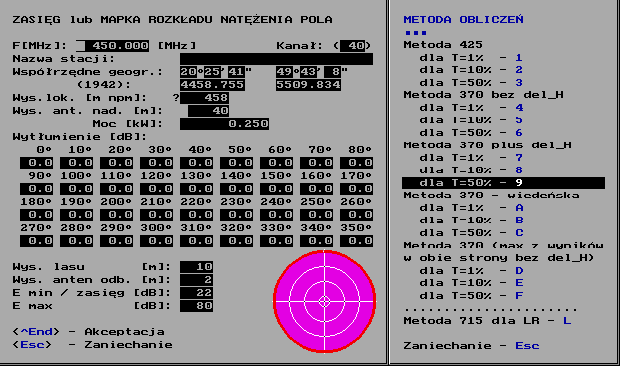
\includegraphics[scale=1]{pics/f1.png}
\caption{Częstotliwość, umieszczenie stacji, wysokość zawieszenia anteny nadawczej, moc nadawania, wysokość anteny odbiorczej oraz wartości E$_{min}$ i E$_{max}$ zaznaczane na mapie}
\end{figure}
\clearpage
\begin{figure}[h!]
\centering
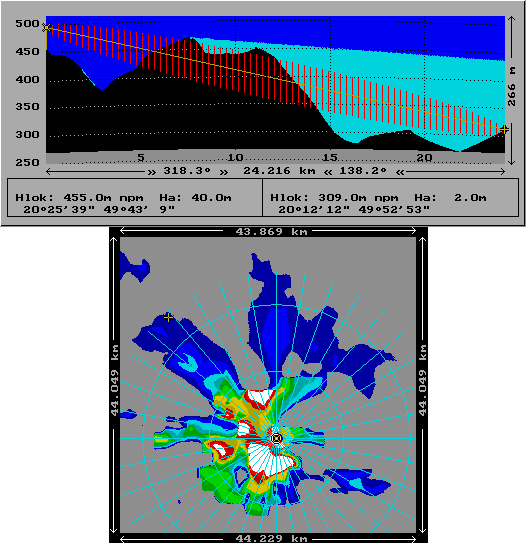
\includegraphics[scale=1]{pics/f2.png}
\caption{Profil terenu oraz mapa z zaznaczoną stacją nadawczą (X) oraz odbiornikiem (+) dla zasięgu maksymalnego NLOS}
\end{figure}
\begin{itemize}
\item Azymut 318 \textdegree.
\item Zasięg max NLOS 24.216 km.
\item Całkowicie przesłonięta 1. strefa Fresnela.
\end{itemize}
\clearpage
\begin{figure}[h!]
\centering
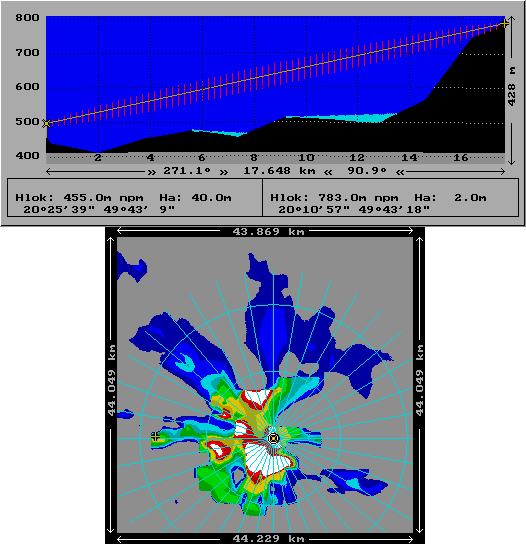
\includegraphics[scale=1]{pics/f3.png}
\caption{Profil terenu oraz mapa z zaznaczoną stacją nadawczą (X) oraz odbiornikiem (+) dla zasięgu maksymalnego LOS}
\end{figure}
\begin{itemize}
\item Azymut 270 \textdegree.
\item Zasięg max NLOS 17.648 km.
\item Całkowicie odsłonięta 1. strefa Fresnela.
\end{itemize}
\clearpage
\begin{figure}[h!]
\centering
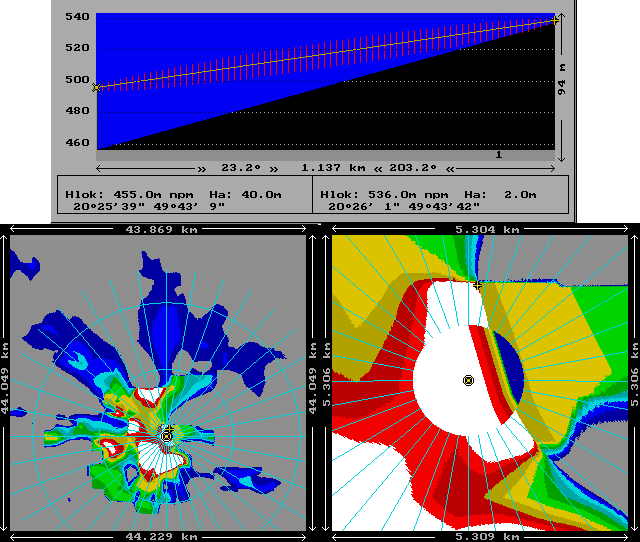
\includegraphics[scale=1]{pics/f4.png}
\caption{Profil terenu oraz mapa z zaznaczoną stacją nadawczą (X) oraz odbiornikiem (+) dla zasięgu minimalnego, a także mapa przedstawiona w przybliżeniu dla dokładniego określenia azymutu}
\end{figure}
\begin{itemize}
\item Azymut 5 \textdegree.
\item Zasięg min 1.137 km.
\item Całkowicie odsłonięta 1. strefa Fresnela.
\end{itemize}
{\bf Pytania:}
\begin{itemize}
\item EIRP = 16 + 8 = 24 [dBW] => EIRP = 250 W.
\item Nadajnik jest przesunięty - niedokładność mapy, ale można poprawić przy wpisywaniu w parametry stacji nadawczej.
\item Wysokość odbiornika 2m.
\item Zasięg max i min LOS/NLOS.
\item Jak porównywać z "Piastem".
\item Co liczyć ręcznie.
\end{itemize}
\end{document}